\documentclass[a4paper,11pt]{article}
\usepackage{graphicx}
\usepackage{lscape}
\usepackage{capt-of}
\usepackage{fancyhdr}
\usepackage{caption}
\usepackage{subcaption}
\usepackage{enumerate}
\usepackage{tikz}
\usetikzlibrary{arrows.meta}
\usepackage{url}
\usepackage{enumerate}
\usepackage{siunitx}
\usepackage{eurosym}
\usetikzlibrary{quotes,angles,positioning}
\usepackage{standalone}
\usepackage{multirow}
\usepackage{url}
\usepackage{float}
\usepackage{geometry} % to change the page dimensions


\newcommand{\subf}[2]{%
  {\small\begin{tabular}[t]{@{}c@{}}
  #1\\#2
  \end{tabular}}%
}  

\geometry{a4paper} 
\pagestyle{fancy}
\lhead{}
\rhead{}
\renewcommand{\headrulewidth}{0pt}
\setlength\parindent{0pt}
\usepackage{amstext} % for \text
\DeclareRobustCommand{\officialeuro}{%
  \ifmmode\expandafter\text\fi
  {\fontencoding{U}\fontfamily{eurosym}\selectfont e}}
\setlength{\parindent}{5ex}

\begin{document}
\begin{titlepage}

\newcommand{\HRule}{\rule{\linewidth}{0.5mm}} % Defines a new command for the horizontal lines, change thickness here

\center % Center everything on the page
 

%----------------------------------------------------------------------------------------
%	TITLE SECTION
%----------------------------------------------------------------------------------------

\HRule \\[0.4cm]
{ \huge \bfseries Network Software Modelling Assignment 2}\\[0.4cm] % Title of your document
\HRule \\[1.5cm]
 
%----------------------------------------------------------------------------------------
%	AUTHOR SECTION
%----------------------------------------------------------------------------------------

\begin{minipage}{0.4\textwidth}
\begin{flushleft} \large
\emph{Students:}\\
Louis \textsc{Carnec} \\% Your name
Vijay \textsc{Katta}\\
Adedayo \textsc{Adelowokan}  
\end{flushleft}
\end{minipage}
~
\begin{minipage}{0.4\textwidth}
\begin{flushright} \large
\emph{Student \#:} \\
15204934 \\ 15202724 \\15204151 % Supervisor's Name
\end{flushright}
\end{minipage}\\[4cm]

% If you don't want a supervisor, uncomment the two lines below and remove the section above
%\Large \emph{Author:}\\
%John \textsc{Smith}\\[3cm] % Your name

%----------------------------------------------------------------------------------------
%	DATE SECTION
%----------------------------------------------------------------------------------------

{\large \today}\\[3cm] % Date, change the \today to a set date if you want to be precise

%----------------------------------------------------------------------------------------
%	LOGO SECTION
%----------------------------------------------------------------------------------------

%\includegraphics{Logo}\\[1cm] % Include a department/university logo - this will require the graphicx package
 
%----------------------------------------------------------------------------------------

{

	 \vspace{1.5in}\textmd{\textbf{Master of Science (Business Analytics)}}\\
     \large{\textbf{UCD Michael Smurfit Graduate Business School }}\\
      \textmd{\textbf{2016-2017}}\\
 }     
\vfill % Fill the rest of the page with whitespace

\end{titlepage}





\section{Real world phenomenon: Spread of disease through airports network} 


The world is more closely connected than ever before by modern transportation networks. Air, sea and land transportation continues to expand in reach, speed of travel and volume of passengers and goods carried. Pathogens and their vectors can now move further, faster and in greater numbers than ever before \cite{tatem2006global}. Epidemics can occur more easily and the emergence of novel pathogens exacerbates the situation \cite{jones2008global}. Understanding the dispersal behaviour and identifying the outbreak of an epidemic in its preliminary stages enables critical response planning. Network topology properties that surround the debut location can explain much of the early stage variation in the spread of diseases \cite{lawyer2016measuring}.

In this simulation we will model the spread of disease through the US airport network. It is inspired by the work of Yager and Taylor \cite{nicholasyager2014} which model the spread of pathogens through airports around the world using a directed graph. We will extend their work by testing how graphs (subgraphs of the US networks graph with specific properties and Erdos-Renyi graphs with different edge existence probabilities) and initial infection nodes (with different centrality measures) affect the spread of disease through the network.

\section{US Airport Network Model}

Our real-world network graph is undirected where nodes represent airports and edges are routes. We used open source data from \url{http://openflights.org}along with population of US cities from \url{https://unstats.un.org/unsd/demographic/products/dyb/City_Page.htm}. Redundant edges and unconnected nodes were removed from the graph. Edge weights were calculates by getting the average population of the two cities connected by edges and normalising for all edges. In creating the graph, only edges connecting airports with the US were added.
The graph created deviates from the real world epidemic scenario. Firstly, exclusively flights within the US are considered. In reality, disease spread through air transport is a world wide phenomenon. In a world wide scenario, we could expect the spread of disease across US nodes to be even quicker as more edges would connect US airport hubs. Secondly, the graph is undirected, this is due to the fact that there is no data for passenger numbers on specific routes. We assume that passenger on routes is proportional to the population of the city which is served by an airport. It is also assumed that routes are bidirectional, to simplify.


\section{Simulation Rules}

The states of each node/airport are either; susceptible to infection (green), infected (yellow) or dead/closed down (red). All nodes are initially disease free and thus susceptible to infection except from a node which is infected at the beginning, step 0. Once a node is infected, it can infect any of its neighbours with probability related to the edge weight connecting it to its neighbours. In the case where the airport can close down or dies (these terms will be used interchangeably), if the airport has closed down it cannot spread anymore disease, there are no outgoing flights. 


Nodes are coloured based on the status - green is susceptible, yellow is infected and red is removed/dead. The four $K_{2,2}$ graphs in Figures \ref{fig:M1} and \ref{fig:M2} below each one represent the state of nodes in a graph at one time step. Figure \ref{fig:M1} (a), demonstrates the initial state, where node A is infected (yellow) and all other nodes are susceptible (green). In Figure \ref{fig:M1} (b), nodes B and D are infected with probabilities ${\emph{w} _{AB}}$  and ${\emph{w}_{DA}}$ respectively, as they are the neighbours of node A. Figure \ref{fig:M2} (a) shows that all nodes are infected and in (b), the next time step, nodes B and D are red, they are dead/closed indefinitely. 

When a node is dead, it cannot further spread the disease. Therefore, if for example the initial node dies before spreading the disease to a neighbour, for example if it has a low probability of spreading the disease, the spread of the disease will be stopped prematurely.

\begin{figure}[H]
\begin{subfigure}{.3\textwidth}
        \centering
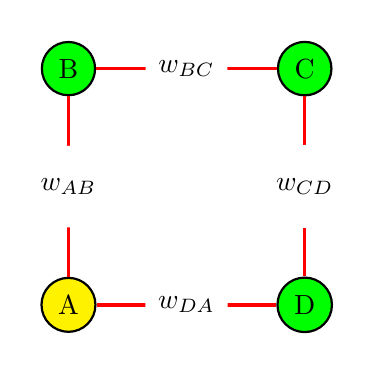
\begin{tikzpicture}
\begin{scope}[every node/.style={circle,thick,draw},local bounding box=aa]
    \node[fill = yellow] (A) at (0,0) {A};
    \node[fill = green] (B) at (0,3) {B};
     \node[fill = green]  (C) at (3,3) {C};
     \node[fill = green]  (D) at (3,0) {D};
\end{scope}

\begin{scope}[>={Stealth[black]},
              every node/.style={fill=white,circle},
              every edge/.style={draw=red,very thick}]
    \path [-] (A) edge node {$w_{AB}$} (B);
    \path [-] (B) edge node {$w_{BC}$} (C);
   \path [-] (C) edge node {$w_{CD}$} (D);
    \path [-] (D) edge node {$w_{DA}$}(A);
\end{scope}
\end{tikzpicture}
\caption{Initial node A infected}
        \label{fig:myfirstsubfig}
    \end{subfigure}%
\begin{subfigure}{.3\textwidth}
        \centering
        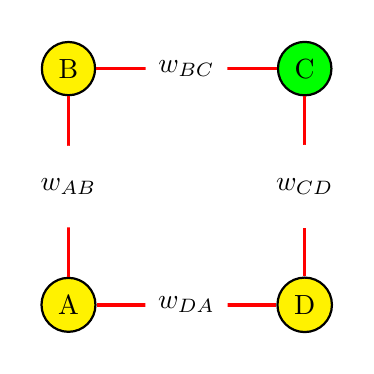
\begin{tikzpicture}
\begin{scope}[every node/.style={circle,thick,draw},shift={(4,0)},local bounding box=bb]
    \node[fill = yellow] (A) at (0,0) {A};
    \node[fill = yellow] (B) at (0,3) {B};
     \node[fill = green]  (C) at (3,3) {C};
     \node[fill = yellow]  (D) at (3,0) {D};
\end{scope}

\begin{scope}[>={Stealth[black]},
              every node/.style={fill=white,circle},
              every edge/.style={draw=red,very thick}]
    \path [-] (A) edge node {$w_{AB}$} (B);
    \path [-] (B) edge node {$w_{BC}$} (C);
   \path [-] (C) edge node {$w_{CD}$} (D);
    \path [-] (D) edge node {$w_{DA}$}(A);
\end{scope}
\end{tikzpicture}
        \caption{B and D infected}
        \label{fig:mysecondsubfig}
    \end{subfigure}
    \caption{Spread of Infection Simulation Rules} \label{fig:M1}
	\end{figure}
\begin{figure}[H]	    
\begin{subfigure}{.3\textwidth}
        \centering
        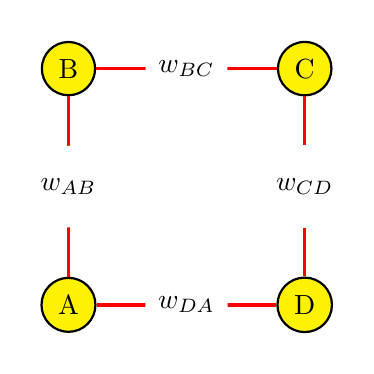
\begin{tikzpicture}
\begin{scope}[every node/.style={circle,thick,draw},shift={(8,0)},local bounding box=bb]
    \node[fill = yellow] (A) at (0,0) {A};
    \node[fill = yellow] (B) at (0,3) {B};
     \node[fill = yellow]  (C) at (3,3) {C};
     \node[fill = yellow]  (D) at (3,0) {D};
\end{scope}

\begin{scope}[>={Stealth[black]},
              every node/.style={fill=white,circle},
              every edge/.style={draw=red,very thick}]
    \path [-] (A) edge node {$w_{AB}$} (B);
    \path [-] (B) edge node {$w_{BC}$} (C);
   \path [-] (C) edge node {$w_{CD}$} (D);
    \path [-] (D) edge node {$w_{DA}$}(A);
\end{scope}
\end{tikzpicture}
        \caption{All nodes infected}
        \label{fig:mysecondsubfig}
    \end{subfigure}
    \begin{subfigure}{.4\textwidth}
        \centering
        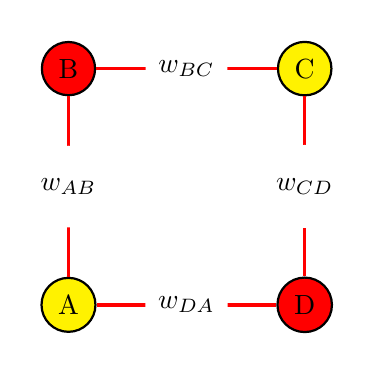
\begin{tikzpicture}
\begin{scope}[every node/.style={circle,thick,draw},shift={(8,0)},local bounding box=bb]
    \node[fill = yellow] (A) at (0,0) {A};
    \node[fill = red] (B) at (0,3) {B};
     \node[fill = yellow]  (C) at (3,3) {C};
     \node[fill = red]  (D) at (3,0) {D};
\end{scope}

\begin{scope}[>={Stealth[black]},
              every node/.style={fill=white,circle},
              every edge/.style={draw=red,very thick}]
    \path [-] (A) edge node {$w_{AB}$} (B);
    \path [-] (B) edge node {$w_{BC}$} (C);
   \path [-] (C) edge node {$w_{CD}$} (D);
    \path [-] (D) edge node {$w_{DA}$}(A);
\end{scope}
\end{tikzpicture}
        \caption{Infected nodes die after n steps}
        \label{fig:mysecondsubfig}
    \end{subfigure}


\caption{Spread of Infection Simulation Rules} \label{fig:M2}
\end{figure}

\section{Simulation and Graph Properties}

\subsection*{Simulation Properties}
We will investigate two main simulation properties; with and without airports being able to close or nodes dying. The hypothesis is that the spread of the disease throughout the network will be slowed down by airport closing as, at each time-step, they cannot spread the disease to neighbours once closed down. \\
Each simulation depends on the probability of being infected at a given timestep ($p_{infection}$) and the time after infection at which the node dies. In both cases $p_{infection} = 0.4$ for simplicity, that is the probability an infected node will infect a neighbour is 0.4, if the edge weight is 1.0. The second simulation, where airports can close, also depends on the time after infection when the airport closes (set in the initial simulation to 4 time steps). We would expect both parameters to have an effect on the spread of disease. The greater the probability of infection, the faster the spread. The longer it takes for the airport to close, the faster the rate of infection. And vice versa. 

\subsection*{Graph Properties}
We hypothesise that the simulations will depend on:

\begin{itemize}
\item Diameter: the largest distance between any two nodes in the graph. The greater the diameter, the longer it should take for the disease to infect the whole graph.
\item Centrality of initial node. The more central an airport/node the faster the disease should spread to other nodes in the network. We will investigate degree centrality and betweenness centrality.
\end{itemize}

\section{Experiments}

The experiments were conducted using 25 time steps, as a result some simulations did not run until the whole graph was infected. Due to the large number of results produced by the experiments, a subset will be presented here.

\subsection*{Testing Diameter Hypothesis}
Both simulations were tested on the airport network and its subgraphs and a range of Erdos-Renyi random graphs for different sizes and probabilities of edge existence. The full US airport graph as a diameter of 4, that is any two airports within the graph have at most 2 airports between them. Subgraphs of the US airport graph are investigated; a subgraph with edge weights $> 0.75$(diameter is infinite, graph not connected), subgraph with edge weights $<0.5$ (diameter = 3), subgraph of 20 largest degree centrality nodes (diameter = 2), and the minimum spanning tree of the airport graph (diameter = 8).\\
Erdos-Renyi graphs' diameter depends on the choice of $n$ (the order of the graph) and $pn$ (probability of an edge existing).

\begin{table}[H]
\centering
\caption{My caption}
\label{my-label}
\begin{tabular}{|l|l|}
\hline
Graph                     & Diameter \\ \hline
\hline
Airport                   & 4        \\ \hline
weights \textgreater 0.75 & inf      \\ \hline
weights\textless0.5       & 3        \\ \hline
High Deg. Cent.           & 3        \\ \hline
Low Deg. Cent.            & 2        \\ \hline
Min. Span. Tree           & 8        \\ \hline
\end{tabular}
\end{table}

\subsection*{Testing Node Centrality}
Tests were also conducted using specific nodes for initial infection based on centrality. The nodes with highest and lowest betweenness and degree centrality, as well as the centre node were infected at time 0 to test their effect on both the real world and Erdos-Renyi graphs.

\section{Results}

\subsection*{Diameter}
\subsubsection*{Airports Graphs and Subgraphs}
The spread of the disease through the graphs differs greatly as we expected depending on the graph we are testing on for both simulations 1 and 2 (see Figures 4,5,12,13). 
In simulation 1, the disease spreads quickly, by the $5^{th}$ timestep, 90\% of the graph is infected but the rate of spread greatly levels out thereafter. Comparing large and low edge weight graphs, the spread for the large edge weight graph is slow whereas it is fast in the low edge weight case. The disease does not spread to the whole graph in the 25 steps of the run but levels out. This has to do with the fact that the whole graph is not connected (diameter = inf). With the 20 largest degree centrality node subgraph, the spread is much quicker than in all other graphs, the disease has spread to the graph in 3 time steps. The minimum spanning tree is slow to spread, it takes some time before the disease reaches a high centrality node, at which point the disease spreading rate increases.\\
Although interesting, these results do not tell much about the effect of graph diameter on disease spread, results are confused with the properties of nodes which make up the subgraphs.

\subsubsection*{Erdos-Renyi}

\subsection*{Node Centrality}

\subsubsection*{Degree Centrality}

\subsubsection*{Betweenness Centrality}


\section{Conclusions}

\section{Appendix}

\documentclass[a4paper&11pt]{article}
\usepackage{caption}
\usepackage{subcaption}
\usepackage{float}
\usepackage[caption = false]{subfig}
\usepackage{graphicx}

\newcommand{\subf}[2]{%
  {\small\begin{tabular}[t]{@{}c@{}}
  #1\\#2
  \end{tabular}}%
}  


\begin{document}
\section*{Simulation 1}

\subsection*{Graphs, subgraph and Edge Probability - Diameter}

\subsubsection*{Erdos-Renyi Graphs}


\begin{table}[H]
\centering
\caption{Simulation 1: Graph properties for different probabilities $pn$ of edge existence between nodes in Erdos-Renyi graphs }
\label{my-label}
\resizebox{\textwidth}{!}{\begin{tabular}{c|c|c|c|c|c|c|c|c}
\hline
index & pn & order & size & density & cluster coefficient &diameter & nodes deg $\geq$ n & largest component \\ \hline
0& 1& 143& 117& 0.011523687580025609& 0.0& inf& 0& 97\\ \hline
1& 3& 143& 325& 0.032010243277848911& 0.03655788655788656& 7& 0& 143\\ \hline
2& 5& 143& 527& 0.051905840638235001& 0.05108083447244284& 5& 14& 143\\ \hline
3& 7& 143& 757& 0.074559243573328077& 0.0733257571774318& 4& 49& 143\\ \hline
4& 9& 143& 885& 0.087166354771988572& 0.08693534635371428& 4& 87& 143\\ \hline
5& 11& 143& 1111& 0.10942578548212351& 0.1088499366852766& 3& 128& 143\\ \hline
\end{tabular}}
\end{table}



\begin{figure}[H]
\centering
\begin{tabular}{|c|c|}
\hline
\subf{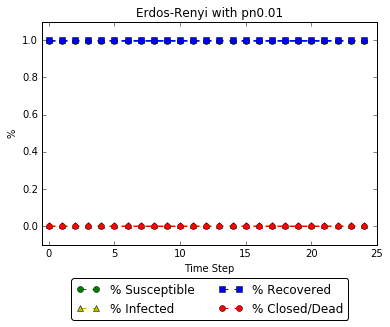
\includegraphics[width=60mm]{ploter01.png}}
     {}
&
\subf{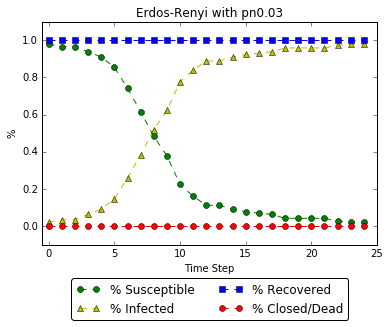
\includegraphics[width=60mm]{ploter03.png}}
     {}
\\
\hline
\subf{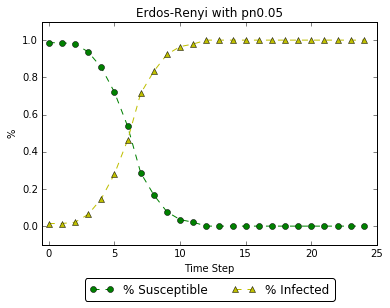
\includegraphics[width=60mm]{ploter05.png}}
     {}
&
\subf{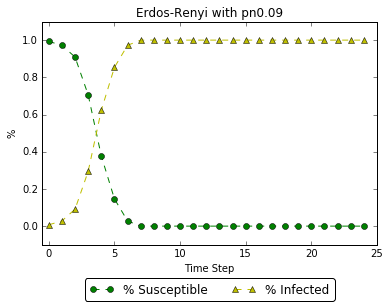
\includegraphics[width=60mm]{ploter09.png}}
     {}
\\
\hline
\end{tabular}
\caption{Simulation 1: Plotting Node States for Erdos Renyi Graphs for pn = 0.1, 0.3, 0.5, 0.9}
\end{figure}

\subsubsection*{Real Airport Graph and subgraphs}

\begin{table}[H]
\centering
\caption{Real World Airport graph and subgraphs graph properties}
\label{my-label}
\resizebox{\textwidth}{!}{\begin{tabular}{c|c|c|c|c|c|c|c}
\hline
Name & order & size & density & cluster coefficient &diameter & nodes deg $\geq$ n & largest component\\ \hline
Real World Graph & 143& 1452& 0.14301191765980498& 0.6410089238208931& 4& 73& 143\\ \hline
Largest Edge Weights &13 & 10 & 0.12820512820512819& 0.0 & inf &1& 7\\ \hline
Lowest Edge Weights & 27 & 102 & 0.29059829059829062 & 0.6458430700260764& 3& 13& 27\\ \hline
20 Largest Deg. Cent. & 20& 177& 0.93157894736842106& 0.9423609156581293& 2& 20& 20\\ \hline
Min Span. Tree & 143& 142& 0.013986013986013986& 0.0& 8& 3& 143\\ \hline
\end{tabular}}
\end{table}

\begin{center}
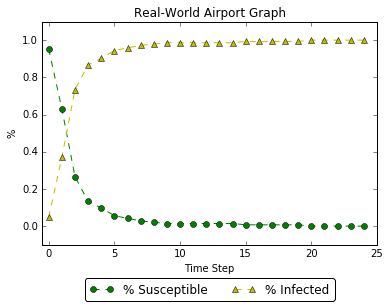
\includegraphics[scale=0.8]{realworldplot.png}
\begin{figure}[H]
\caption{Simulation1: Real-world airport graph properties}
\end{figure}
\end{center}


\begin{figure}[H]
\centering
\begin{tabular}{|c|c|}
\hline
\subf{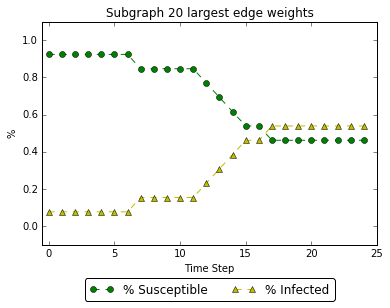
\includegraphics[width=60mm]{sublargedgewsim1.png}}
     {}
&
\subf{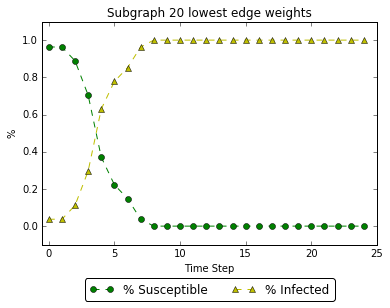
\includegraphics[width=60mm]{sublowestedgewsim1.png}}
     {}
\\
\hline
\subf{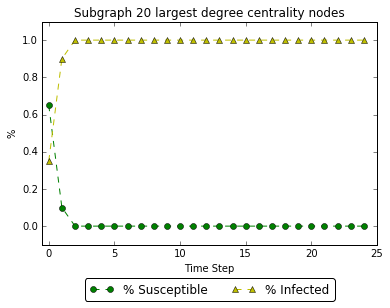
\includegraphics[width=60mm]{largestdegcsim1.png}}
     {}
&
\subf{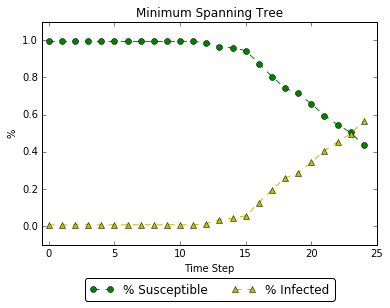
\includegraphics[width=60mm]{minspansim1.png}}
     {}
\\
\hline
\end{tabular}
\caption{Simulation 1: Subgraph node state plots}
\end{figure}

\subsection*{Source Node Centrality}
\subsubsection*{Erdos-Renyi Graph with p = ??}
\subsubsection*{Real World Graph}

%
%Begin: Sim1 - Real 
\begin{center}
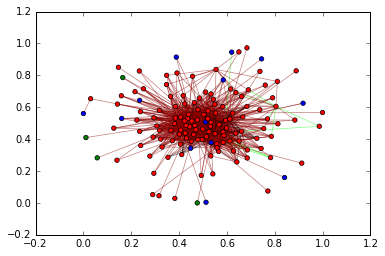
\includegraphics[scale=0.8]{11InitialNode_Center_of_graph_1.png}
\begin{figure}[H]
\caption{Simulation1: Initial Node Center Of Graph }
\end{figure}
\end{center}

\begin{center}
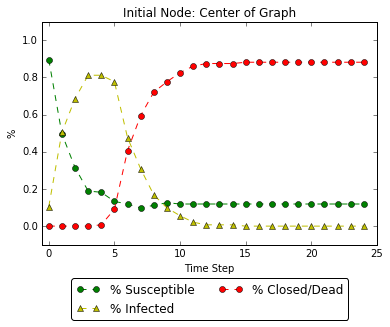
\includegraphics[scale=0.8]{11InitialNode_Center_of_graph_2.png}
\begin{figure}[H]
\caption{Simulation1: Initial Node Center Of Graph - Statistics}
\end{figure}
\end{center}


\begin{figure}[H]
\centering
\begin{tabular}{|c|c|}
\hline
\subf{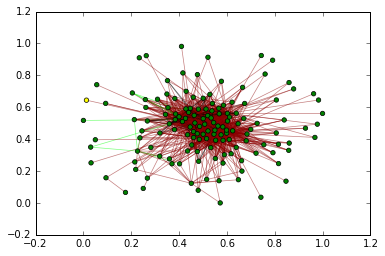
\includegraphics[width=60mm]{11MinDegree_Centrality_source_node_1.png}}
     {}
&
\subf{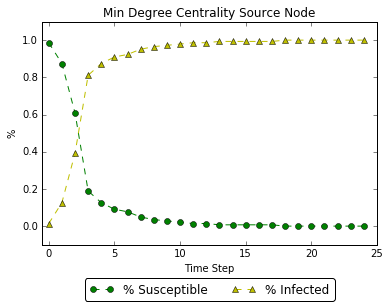
\includegraphics[width=60mm]{11MinDegree_Centrality_source_node_2.png}}
     {}
\\
\hline
\subf{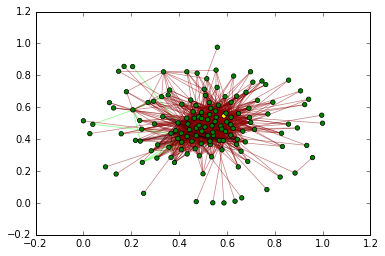
\includegraphics[width=60mm]{11MaxDegree_Centrality_source_node_1.png}}
     {}
&
\subf{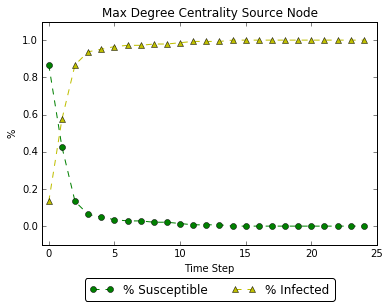
\includegraphics[width=60mm]{11MaxDegree_Centrality_source_node_2.png}}
     {}
\\
\hline
\end{tabular}
\caption{Simulation 1: Max and Min Degree Centrality SourceNode}
\end{figure}


\begin{figure}[H]
\centering
\begin{tabular}{|c|c|}
\hline
\subf{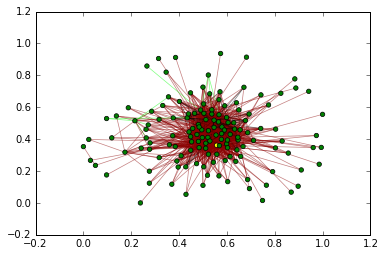
\includegraphics[width=60mm]{11MaxBetweeness_centrality_sourcenode_1.png}}
     {}
&
\subf{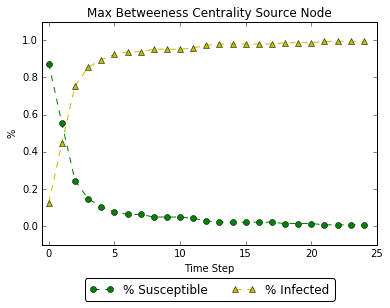
\includegraphics[width=60mm]{11MaxBetweeness_centrality_sourcenode_2.png}}
     {}
\\
\hline
\subf{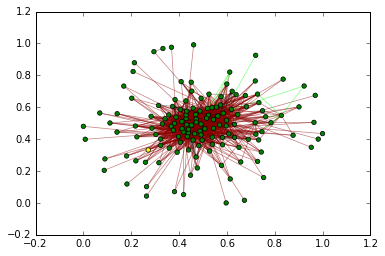
\includegraphics[width=60mm]{11MinBetweeness_centrality_sourcenode_1.png}}
     {}
&
\subf{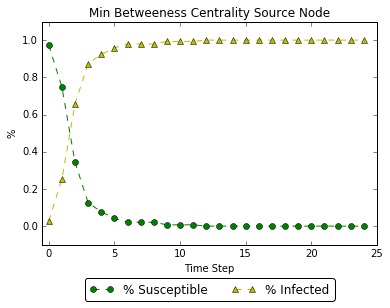
\includegraphics[width=60mm]{11MinBetweeness_centrality_sourcenode_2.png}}
     {}
\\
\hline
\end{tabular}
\caption{Simulation 1: Max and Min Betweenness Centrality SourceNode}
\end{figure}

%End: Sim1 - Real 

%Begin: Sim2 - Real 
\begin{center}
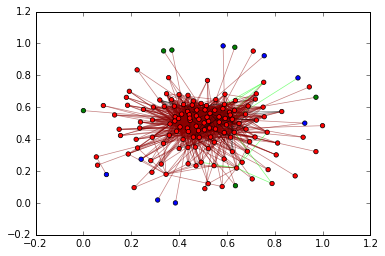
\includegraphics[scale=0.8]{InitialNode_Center_of_graph_1.png}
\begin{figure}[H]
\caption{Simulation2: Initial Node Center Of Graph }
\end{figure}
\end{center}

\begin{center}
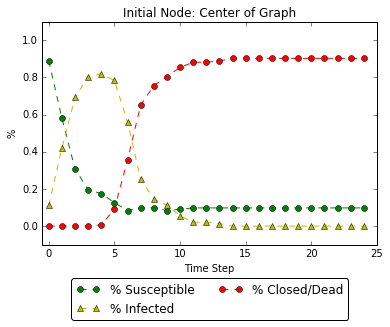
\includegraphics[scale=0.8]{InitialNode_Center_of_graph_2.png}
\begin{figure}[H]
\caption{Simulation2: Initial Node Center Of Graph - Statistics}
\end{figure}
\end{center}


\begin{figure}[H]
\centering
\begin{tabular}{|c|c|}
\hline
\subf{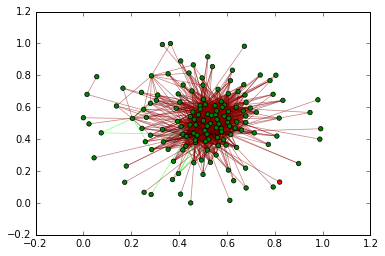
\includegraphics[width=60mm]{MinDegree_Centrality_source_node_1.png}}
     {}
&
\subf{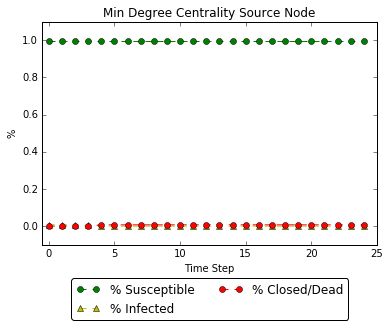
\includegraphics[width=60mm]{MinDegree_Centrality_source_node_2.png}}
     {}
\\
\hline
\subf{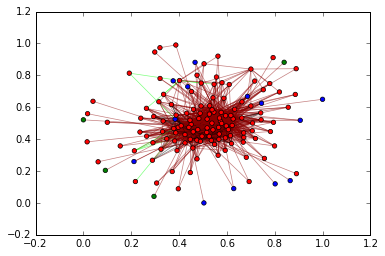
\includegraphics[width=60mm]{MaxDegree_Centrality_source_node_1.png}}
     {}
&
\subf{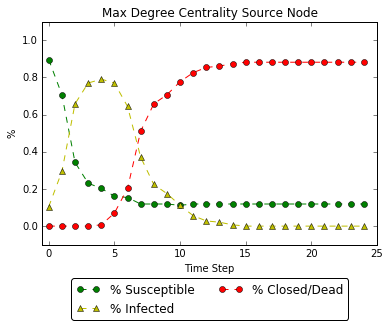
\includegraphics[width=60mm]{MaxDegree_Centrality_source_node_2.png}}
     {}
\\
\hline
\end{tabular}
\caption{Simulation 2: Max and Min Degree Centrality SourceNode}
\end{figure}


\begin{figure}[H]
\centering
\begin{tabular}{|c|c|}
\hline
\subf{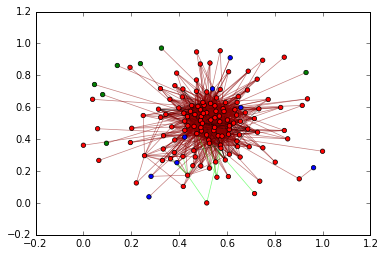
\includegraphics[width=60mm]{MaxBetweeness_centrality_sourcenode_1.png}}
     {}
&
\subf{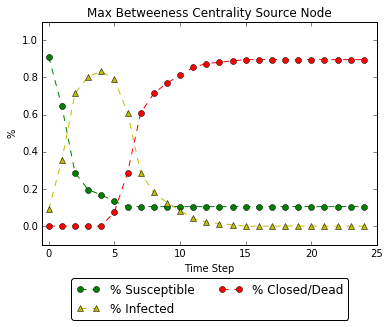
\includegraphics[width=60mm]{MaxBetweeness_centrality_sourcenode_2.png}}
     {}
\\
\hline
\subf{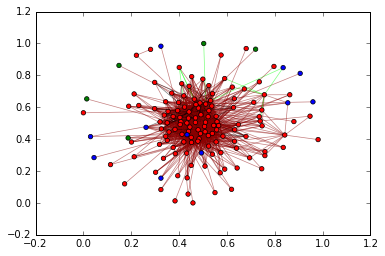
\includegraphics[width=60mm]{MinBetweeness_centrality_sourcenode_1.png}}
     {}
&
\subf{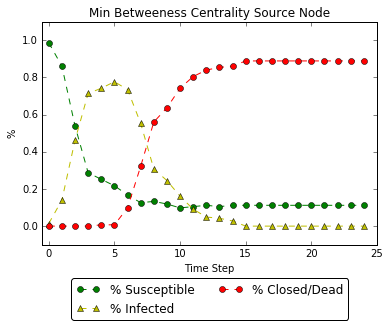
\includegraphics[width=60mm]{MinBetweeness_centrality_sourcenode_2.png}}
     {}
\\
\hline
\end{tabular}
\caption{Simulation 2: Max and Min Betweenness Centrality SourceNode}
\end{figure}

%End: Sim2 - Real 

\section*{Simulation 2}
\subsection*{Erdos-Renyi Graphs}


\begin{table}[H]
\centering
\caption{Simulation 2: Erdos Renyi Graph properties for pn = 0.1, 0.3, 0.5, 0.9}
\label{my-label}
\resizebox{\textwidth}{!}{\begin{tabular}{c|c|c|c|c|c|c|c|c}
\hline
index & pn & order & size & density & cluster coefficient &diameter & nodes deg $\geq$ n & largest component\\ \hline
0& 1& 143& 103& 0.010144784792672116& 0.008857808857808859& inf& 0& 81\\ \hline
 1& 3& 143& 310& 0.030532847434255887& 0.017199467199467203& inf& 0& 141\\ \hline
 2& 5& 143& 530& 0.052201319806953611& 0.045021276314982595& 5& 12& 143\\ \hline
 3& 7& 143& 734& 0.072293903279818772& 0.07440109217101569& 4& 49& 143\\ \hline
 4& 9& 143& 889& 0.087560326996946714& 0.09322985284361361& 4& 86& 143\\ \hline
 5& 11& 143& 1162& 0.1144489313503398& 0.11609641591068731& 3& 128& 143\\ \hline
\end{tabular}}
\end{table}


\begin{figure}[H]
\centering
\begin{tabular}{|c|c|}
\hline
\subf{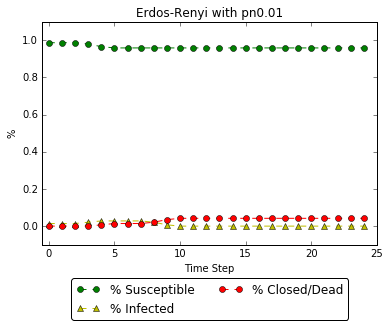
\includegraphics[width=60mm]{plotdie01.png}}
     {}
&
\subf{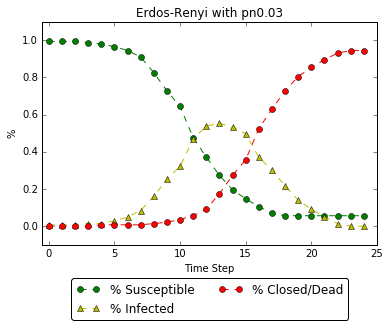
\includegraphics[width=60mm]{plotdie03.png}}
     {}
\\
\hline
\subf{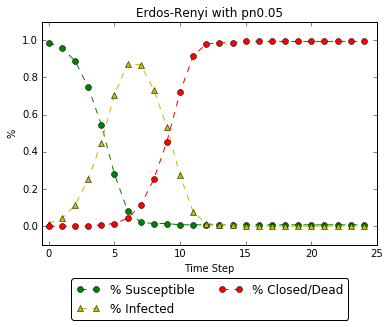
\includegraphics[width=60mm]{plotdie05.png}}
     {}
&
\subf{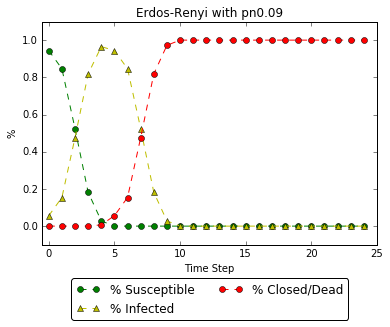
\includegraphics[width=60mm]{plotdie09.png}}
     {}
\\
\hline
\end{tabular}
\caption{Simulation 2: Plotting Node States for Erdos Renyi Graphs for pn = 0.1, 0.3, 0.5, 0.9}
\end{figure}

\subsubsection*{Real Airport Graph and subgraphs}




\begin{center}
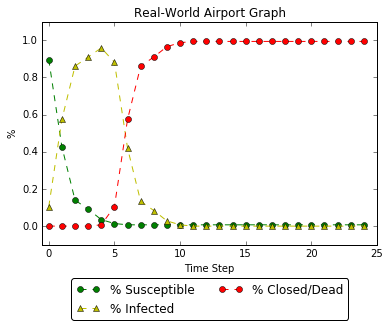
\includegraphics[scale=0.8]{realworldplotsim2.png}
\begin{figure}[H]
\caption{Simulation 2: Real-world airport graph properties}
\end{figure}
\end{center}

\begin{figure}[H]
\centering
\begin{tabular}{|c|c|}
\hline
\subf{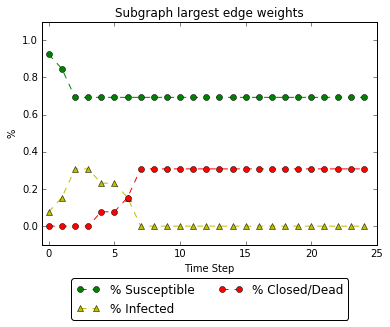
\includegraphics[width=60mm]{largestedgesim2.png}}
     {}
&
\subf{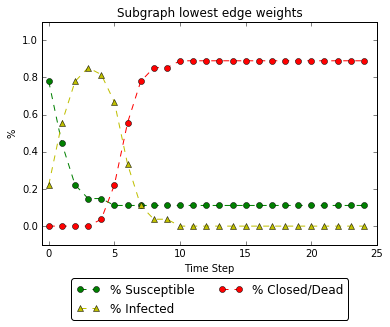
\includegraphics[width=60mm]{lowestedgesim2.png}}
     {}
\\
\hline
\subf{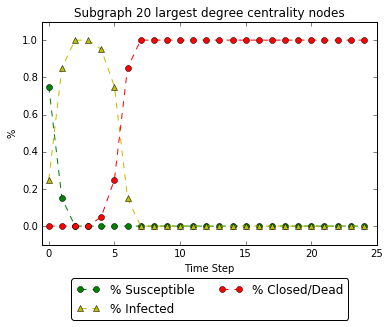
\includegraphics[width=60mm]{largestsim2.png}}
     {}
&
\subf{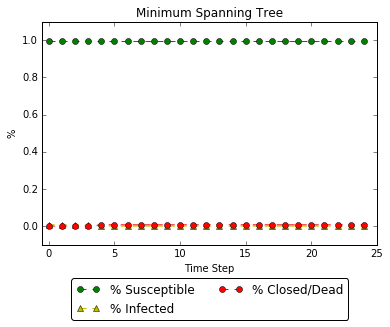
\includegraphics[width=60mm]{minspantreesim2.png}}
     {}
\\
\hline
\end{tabular}
\caption{Simulation 2: Plotting Node States for Erdos Renyi Graphs for pn = 0.1, 0.3, 0.5, 0.9}
\end{figure}


\subsection*{Source Node Centrality}
\subsubsection*{Erdos-Renyi Graph with p = ??}
\subsubsection*{Real World Graph}

\end{document}

















\end{document}

